\section{Language Structure}
\label{sec:LanguageStructure}
This section defines how you express a state machine or system of state
machines. A Moore machine can be defined using a set of six items. These are:

\begin{itemize}
   \item Finite set of states (S)
   \item Initial state ($S_0$)
   \item Finite input alphabet ($\Sigma$)
   \item Finite ouitput alphabet ($\Lambda$)
   \item Transition function ($T:S\times\Sigma\rightarrow S$)
   \item Output function ($G:S \rightarrow \Lambda$)
\end{itemize}

Graphically this is shown below in Figure \ref{fig:MooreMachine}.

\begin{figure}[h]
   \centering
   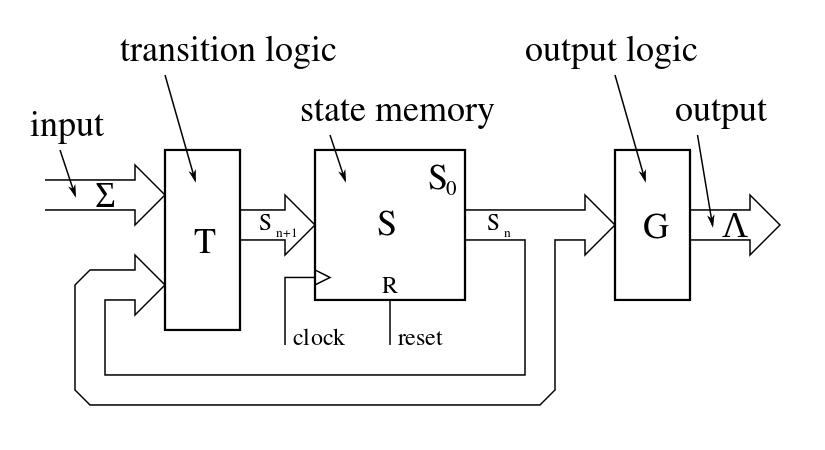
\includegraphics[scale=0.4]{MooreMachine}
   \caption{Moore Machine}
   \small{Taken from:://commons.wikimedia.org/wiki/File:Moore-Automat-en.svg}
   \label{fig:MooreMachine}
\end{figure}
\FloatBarrier

\subsection{State Machine Syntax}
The structure of a state machine is shown in the code below. It describes the
six parts of a Moore machine described in Section \ref{sec:LanguageStructure}
Language Structure.

\lstinputlisting{StateMachineExample.sm}

\subsection{System Syntax}
The purpose of a system is to be able to connect multiple state machines or
systems together. The structure is shown in the code below.

\lstinputlisting{SystemExample.sm}
